\section{Symmetry}
\label{sec:symmetry}
\begin{center}
\begin{large}
 \textbf{This functionality is considered "under development". Please report any errors to the \textit{aimsclub}.\\ No post-processing (DOS, band-structure) implemented, yet. Only realspace EXX.}
\end{large}
\end{center}

\textit{FHI-aims} can make use of symmetry to reduce the number of k-points and thus the number of calls to the eigensolver. The functionality is based on the external library \textit{spglib} written by Atsushi Togo (\textbf{https://atztogo.github.io/spglib/}). For instructions how-to compile \textit{FHI-aims} with \textit{spglib} see Appendix \ref{app:spglib}.\\
\begin{figure}
\centering
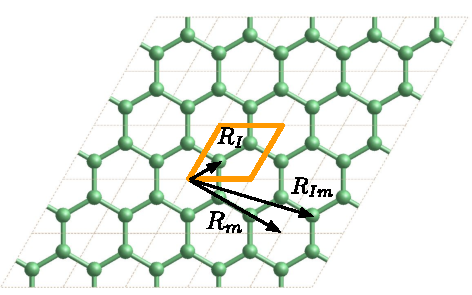
\includegraphics[width=0.75\textwidth]{lattice.pdf}
\caption{\label{fig1}. Illustration of atomic coordinates in the unit cell ($\mathbf{R}_{I}$), lattice vector ($\mathbf{R}_m$) and atomic coordinates in super cell ($\mathbf{R}_{Im}=\mathbf{R}_{I}+\mathbf{R}_m$). Image credits: Honghui Shang.}
\end{figure}
In real space, {\it FHI-aims} uses the Bloch functions
\begin{equation}
 \varphi_{I(\mu),\mathbf{k}}(\mathbf{r})=\sum_m\chi_{I(\mu),m}(\mathbf{r})\exp(-i\mathbf{k}\mathbf{R}_m) \;,
 \label{Bloch}
\end{equation}
where
\begin{equation}
\chi_{I(\mu),m}(\mathbf{r})=\chi_{I(\mu),m}(\mathbf{r}-\mathbf{R}_{I(\mu)}-\mathbf{R}_m)\label{localbase}
\end{equation}
is the local basis function (atomic orbital) with the quantum numbers~$\mu=(n,l,m)$ associated with atom $I(\mu)$ in the $m^\text{th}$~periodic replica of the unit cell~(see Fig.~\ref{fig1}). The general space group symmetry operator has the form:
\begin{equation}
 \hat{S}=\{V|\mathbf{R}+\mathbf{f}\}
\end{equation}
$V$ are rotations, $\mathbf{f}$ (fractional) translation vectors and $\mathbf{R}$ direct lattice translation vectors. Under such symmetry operations
$\{V|\mathbf{f}\}$, the local basis function in equation~\ref{localbase} transform according to:
\begin{align}
\{V|\mathbf{f}\}\chi_{I(\mu),m}(\mathbf{r})=&\\\chi_{I(\mu),m}(V^{-1}\mathbf{r}-
&V^{-1}(\mathbf{R}_{I(\mu)}+\mathbf{R}_m+\mathbf{f})) \;.
\end{align}
We make use of the fact that Atom $I$ of the first unit cell is transformed by application of ${V^-1|\mathbf{f}}$ into atom $J$ in the $j$th unit cell. Also, $\mathbf{O}_I^V$ is the vector translating $\mathbf{R}_{J(\mu)}$ back to the first unit cell ($V^{-1}(\mathbf{R}_{I(\mu)}-\mathbf{f})\rightarrow \mathbf{R}_{J,c}; \mathbf{O}_I^V = \mathbf{R}_{J,0} - \mathbf{R}_{J,c}$): 
\begin{eqnarray}
 \mathbf{R}_{I(\mu)}+\mathbf{R}_m & = & V(\mathbf{R}_{I(\mu)}^V+\mathbf{R}_m^V)+\mathbf{f} \\
 \mathbf{R}_{I(\mu)}^V            & = & V^{-1}(\mathbf{R}_{I(\mu)}-\mathbf{f})+\mathbf{O}_I^V=\mathbf{R}_{J(\mu')}\label{RItoJ} \\
 \mathbf{R}_m^V                   & = & V^{-1}\mathbf{R}_m-\mathbf{O}_I^V=\mathbf{R}_j
\end{eqnarray}
Using this, we finally get:
\begin{equation}
\{V|\mathbf{f}\}\chi_{I(\mu),m}(\mathbf{r})=\sum_{m'}\hat{T}(V,l,m,m')\chi_{J(\mu'),j}(\mathbf{r}-\mathbf{R}_{J(\mu')}-\mathbf{R}_j) \;,
\end{equation}
in which $\hat{T}(V,l,m,m')$ is the transformation matrix of the spherical harmonics $Y_{lm}$. 
Along the same line, the Bloch states in Eq.~(\ref{Bloch}) fulfill
\begin{equation}
 \mathbf{k}\mathbf{R}_m = (V^{-1}\mathbf{k})(V^{-1}\mathbf{R}_m+\mathbf{O}_I^V-\mathbf{O}_I^V)=\mathbf{k}^V\mathbf{R}_m^V+\mathbf{k}^V \mathbf{O}_I^V
\end{equation}
so that we get
\begin{equation}
 \{V|\mathbf{f}\}\varphi_{I(\mu),\mathbf{k}}(\mathbf{r})= \exp\left(-i\mathbf{k}^{V}\mathbf{O}_I^V\right)\sum_{m'}\hat{T}(V,l,m,m')\varphi_{J(\mu'),\mathbf{k}^V}(\mathbf{r})
\end{equation}
Please note that the
KS eigen-coefficients transform exactly like the basis functions:
\begin{align}
c_{i,I(\mu),\mathbf{k}}    = \exp(-i\mathbf{k}^{V}\mathbf{O}_I^V)\sum_{m'}\hat{T}(V,l,m,m')c_{i,J(\mu'),\mathbf{k}^V}\\
c_{i,J(\mu'),\mathbf{k}^V} = \exp(i\mathbf{k}^{V}\mathbf{O}_I^V)\sum_{m}\hat{T}^{+}(V,l,m,m')c_{i,I(\mu),\mathbf{k}}\label{cij_trafo}
\end{align}

The symmetry analysis, k-point reduction and reconstruction of the density matrix is done as follows:
\begin{enumerate}
 \item[1.] We use \textit{spglib} (http://atztogo.github.io/spglib/) to
\begin{itemize}
 \item determine the space group of the system               
 \item determine translation vectors ($\mathbf{f}$) and rotation matrices ($V$) for this space group
\end{itemize}
See Appendix \ref{app:spglib} how-to include \textit{spglib} during the compilation of \textit{FHI-aims}.  
Additionally, we implemented routines to
\begin{itemize}
 \item tabulate the rotation matrices ($V$) required for the calculation of $\hat{T}(V,l,m,m')$.
 \item and calculate the distance $\mathbf{O}$ between equivalent atoms due to the symmetry operation $\{V|\mathbf{f}\}$ to determine the phase factor in Eq.~\ref{cij_trafo}.
 \item determine the equivalent $\mathbf{k}$-points 
 \item construct the map between symmetry-equivalent $\mathbf{k}$-points
\end{itemize}
 \item[2.] The Euler angles are calculated from the rotation matrices~$V(\alpha,\beta,\gamma)$.
    \begin{align*}
    &V(\alpha,\beta,\gamma)=\\
    &\left(\begin{matrix}
     \cos\gamma\cos\beta\cos\alpha-\sin\gamma\sin\alpha &
     \cos\gamma\cos\beta\sin\alpha+\sin\gamma\cos\alpha &
    -\cos\gamma\sin\beta \\
    -\sin\gamma\cos\beta\cos\alpha-\cos\gamma\sin\alpha &
    -\sin\gamma\cos\beta\sin\alpha+\cos\gamma\cos\alpha &
     \sin\gamma\sin\beta \\
     \sin\beta\cos\alpha &
     \sin\beta\sin\alpha &
     \cos\beta
    \end{matrix}\right),
   \end{align*}
This  corresponds to the ``y-convention'':
   \begin{itemize}
    \item[1.]{The $x_1'$-, $x_2'$-, $x_3'$-axes are rotated anticlockwise
     through an angle $\alpha$ about the $x_3$ axis}
    \item[2.]{The $x_1''$-, $x_2''$-, $x_3''$-axes are rotated anticlockwise
     through an angle $\beta$ about the $x_2'$ axis}
    \item[3.]{The $x_1'''$-, $x_2'''$-, $x_3'''$-axes are rotated anticlockwise
     through an angle $\gamma$ about the $x_3''$ axis}
   \end{itemize}
 \item[3.] The rotation matrices~$\hat{T}(V,l,m,m')=\hat{T}(V(\alpha,\beta,\gamma),l,m,m')=\hat{T}^l_{m,m'}(\alpha,\beta,\gamma)$ for the \textbf{real} spherical harmonics ($\hat{T}(V,l,m,m')$)
 are calculated.\\
 The rotation matrix in the basis of the \textbf{real} spherical harmonics is calculated from the rotation matrix in the basis of the \textbf{complex} spherical harmonics, the Wigner D-Matrix~$D^l_{mm'}(\alpha,\beta,\gamma)$, and a transformation matrix~$\hat{C}^l_{m,m'}$ (see \textit{M. A. Blanco, M. Florez, M. Bermejo, J. of Mol. Strucure, 419 (1997) 19-27}, \cite{Blanco1997}):
 \begin{align*}
  \hat{T}^l_{m,m'}(\alpha,\beta,\gamma)=\hat{C}^{l\quad *}_{m,m'}\hat{D}^l_{mm'}(\alpha,\beta,\gamma)\hat{C}^{l\quad T}_{m,m'}
 \end{align*}
 \begin{itemize}
  \item The Wigner D-Matrix (rotation matrix in the basis of the \textbf{complex} spherical harmonics ) is defined by the formula:
    \begin{align*}
    D^l_{mm'}(\alpha,\beta,\gamma)&=\sum_i\frac{(-1)^i\sqrt{(l+m)!(l-m)!(l+m')!
    (l-m')!}}{(l-m'-i)!(l+m-i)!i!(i+m'-m)!}\\
    &\times\left(\cos\frac{\beta}{2}\right)^{2l+m-m'-2i}\left(\sin\frac{\beta}
    {2}\right)^{2i+m'-m}e^{-i(m\alpha+m'\gamma)},
   \end{align*}
   (from ``Bradley and Cracknell, The mathematical theory of symmetry in solids : representation theory for point groups and space groups, Clarendon Pr., 1972, p.53'', \cite{Cracknell1972})
  Thereby, improper rotations (combination of rotation and inversion) are made proper $R\rightarrow-R$ and $D^l_{mm'}\rightarrow(-1)^l D^l_{mm'}$. In practice the calculation of $D^l_{mm'}(\alpha,\beta,\gamma)$ is done with a recursive algorithm, that does not require the calculation of factorials.~(\textit{M. A. Blanco, M. Florez, M. Bermejo, J. of Mol. Strucure, 419 (1997) 19-27}, \cite{Blanco1997})
 \item 
 $\hat{C}^l_{m,m'}$ is constructed by these 6 rules:
 \begin{enumerate}
  \item[1.] $\hat{C}^l_{m,m'}=0$ if $|m|\neq|m'|$
  \item[2.] $\hat{C}^l_{0,0}=1$
  \item[3.] $\hat{C}^l_{m,m}=(-1)^m/\sqrt{2}$
  \item[4.] $\hat{C}^l_{m,-m}=1/\sqrt{2}$
  \item[5.] $\hat{C}^l_{-m,m}=-\text{i}(-1)^m/\sqrt{2}$
  \item[6.] $\hat{C}^l_{-m,-m}=\text{i}/\sqrt{2}$
 \end{enumerate}
 \item Last but not least, we have to take care of the sign convention for the real spherical harmonics as implemented in FHI-aims -- figuring this out took us some time. In practice, this is taken care of by an additional matrix multiplication (with  $T^l_{m,m'}$) yielding the correct signs in $\hat{C}^l_{m,m'}$.
 \begin{align*}
  \hat{C}^l_{m,m'}= T^l_{m,m'}\times \hat{C}^l_{m,m'}
 \end{align*}
\end{itemize}
\item[4.] Eventually, this matrices are used to transform the KS eigen-coefficients following Eq.~(\ref{cij_trafo}).
Furthermore, the rotation of the KS-eigenvectors can be made more efficient 
by directly transforming the density matrix $n(\mathbf{k},n,m)$ at each k-point with the help of two 
matrix operations:
\begin{align}
\label{mm_reconstruction}
 n(\mathbf{k},n,m)=\sum_{i,j}^{occ}c^*_{i,n,\mathbf{k}}c_{j,m,\mathbf{k}}=&\sum_{i,j}^{occ}\sum_{n'}exp(i\mathbf{k}^{V}\mathbf{O}_{n'}^V)T^*_{n,n'}c^*_{i,n',\mathbf{k}^V}\\
 &\times \sum_{m'}exp(-i\mathbf{k}^{V}\mathbf{O}_{m'}^V)T_{m,m'}c_{j,m',\mathbf{k}^V}\nonumber\\
 &=\hat{T}^* n(\mathbf{k}^V,n',m') \hat{T}^T\nonumber
\end{align}
The phase factor $exp(i\mathbf{k}^{V}\mathbf{O}_{n'}^V)$ can be included in the transformation matrix during the pre-processing. This increases the matrix size (and required memory) by a factor of the size of the number of k-points to reconstruct at each computing task. Furthermore the density matrix only has to be reconstructed for k-points reduced by proper rotations. The corresponding improper (inversion symmetry) rotations are accounted for by the integration weights.
\end{enumerate}
\newpage


\subsection*{Tags for general section of \texttt{control.in}:}

\keydefinition{symmetry\_reduced\_k\_grid\_spg}{control.in}
{
  \noindent
  Usage: \keyword{symmetry\_reduced\_k\_grid\_spg} \option{.true./.false.}\\[1.0ex]
  Purpose: Only use the irreducible set of k-points during the calculation. Default: \option{.false.}
  \\[1.0ex]
}

\keydefinition{reconstruct\_proper\_only}{control.in}
{
  \noindent
  Usage: \keyword{reconstruct\_proper\_only} \option{.true./.false.}\\[1.0ex]
  Purpose: Only reconstruct the density matrix for proper rotations. Improper rotations (Inversion symmetry) are accounted for by the integration weights. Default: \option{.true.} 
  \\[1.0ex]
}

\keydefinition{use\_spg\_full\_Delta}{control.in}
{
  \noindent
  Usage: \keyword{use\_spg\_full\_Delta} \option{.true./.false.}\\[1.0ex]
  Purpose: Include phase factors in the reconstruction matrix for the density matrix during pre-processing. Set to \option{.false.} if memory is an issue. Default: \option{.true.} 
  \\[1.0ex]
}

\keydefinition{use\_spg\_mv\_mm}{control.in}
{
  \noindent
  Usage: \keyword{use\_spg\_mv\_mm} \option{.true./.false.}\\[1.0ex]
  Purpose: Reconstruct the density by rotating the eigenvector and setting up the density matrix in the standard way (matrix-vector and matrix-matrix operation instead of the matrix-matrix operations in Eq.~\ref{mm_reconstruction}). Default: \option{.false.} 
  \\[1.0ex]
}

\keydefinition{use\_symmetric\_forces}{control.in}
{
  \noindent
  Usage: \keyword{use\_symmetric\_forces} \option{.true./.false.}\\[1.0ex]
  Purpose: Symmetrize the forces and generalized forces on the lattice, i.\,e., 
  the stress, for geometry relaxation, e.\,g., to preserve crystal symmetry but 
  without fully reducing the k-point set. If full symmetry is used for k-point 
  reduction, forces are symmetrized. The forces are symmetrized by averaging 
  over all symmetry operations. Default: \option{.false.} 
  \\[1.0ex]
}
